\subsection{`SET': grouping and compositionality in relational reasoning}\label{ssec:experiments_set}

`SET' is a card game which forms a simple but challenging relational task. The `objects' are a set cards each representing four attributes which can take one of three values each. `Color' can be red, green, or purple; `number' can be one, two, or three; `shape' can be diamond, squiggle, or oval; and `fill' can be solid, striped, or empty. A `set' is a triplet of cards such that each attribute is either the same on all three cards or different on all three cards.~\Cref{fig:contains_set_example} shows a sample of SET cards.

% \begin{wrapfigure}{R}{0.25\textwidth}
% 	% \vskip-5pt
% 	\begin{tabular}{c}
% 		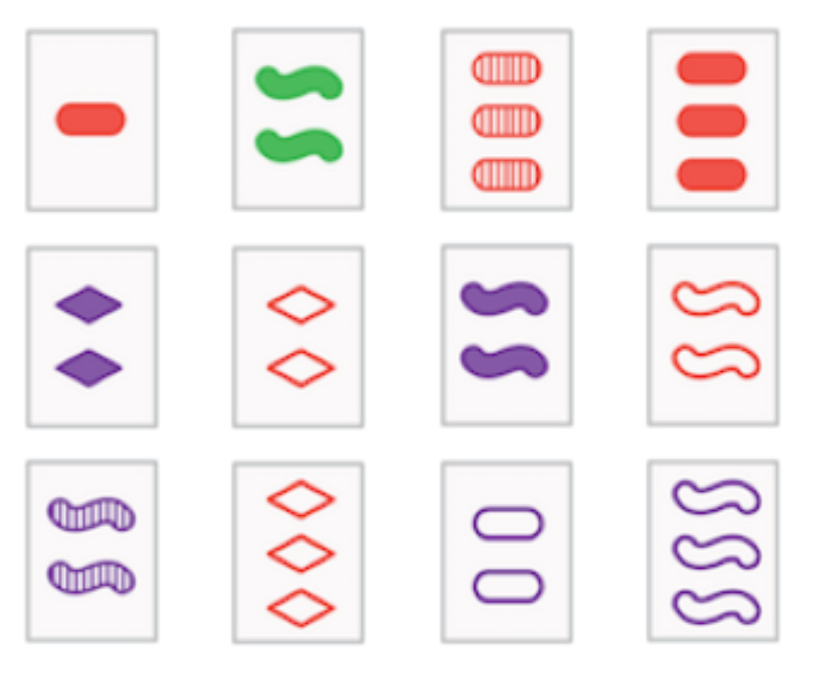
\includegraphics[width=.25\textwidth]{figs/set_example}\\[-5pt]
% 	\end{tabular}
% 	\caption{\footnotesize The SET game}\label{fig:set_example}
% \end{wrapfigure}
In SET, the task is: given a hand of $k > 3$ cards, find a `set' among them (typically, SET is played with $k=12$, with two players competing to find a `set' first). This task is deceptively challenging, and is representative of the type of relational reasoning that humans excel at but machine learning systems still struggle with. To solve the task, one must process the sensory information of individual cards to identify the values of each attribute, then somehow search over combinations of cards and reason about the relations between them. Importantly, this type of relational reasoning requires attending over several attributes and relations simultaneously while representing some notion of `groups'.  The construct of relational convolutions proposed in this paper is a step towards developing machine learning systems which can perform this kind of relational reasoning.


In this section, we evaluate RelConvNet on a task based on `SET' and compare it to several baselines. The task is: given a sequence of $k=5$ images of SET cards, determine whether or not they contain a `set'. All models share the common architecture $(x_1, \ldots, x_k) \to \texttt{CNN} \to \{ \cdot \} \to \texttt{MLP} \to \hat{y}$, where $\{\cdot\}$ indicates the model being tested. In addition to CoRelNet, PrediNet, and Transformers, we also compare RelConvNet to GNN and RNN baselines. The architectural details can be found in~\Cref{tab:set_architectures}. The CNN embedder is pre-trained on the task of classifying the four attributes of the cards and an intermediate layer is used to generate embeddings of dimension $64$ for each card. The output MLP architecture is shared across all models, and consists of two hidden layers with $64$ and $32$ neurons, respectively, and ReLU activations.

% \begin{wrapfigure}{R}{0.375\textwidth}
%     \centering
%     % \vskip-10pt
%     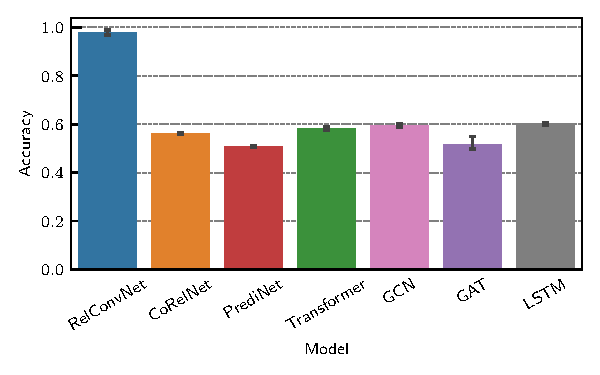
\includegraphics[width=0.375\textwidth]{figs/experiments/contains_set_acc.pdf}\\[-5pt]
%     \caption{\footnotesize{Hold-out test accuracy. Error bars indicate 95\% bootstrap confidence intervals.}}\label{fig:contains_set_acc}
% \end{wrapfigure}

In SET, there exists $\binom{81}{3} = 85\,320$ triplets of cards, of which $1\,080$ are a `set'. We partition the `sets' into training (70\%), validation (15\%), and test (15\%) sets. The training, validation, and test datasets are generated by sampling $k$-tuples of cards such that with probability $1/2$ the $k$-tuple does not contain a set, and with probability $1/2$ it contains a set among the corresponding partition of sets. Partitioning the data in this way allows us to measure the models' ability to ``learn the rule'' and identify new unseen `sets'. We train for 100 epochs with the same loss, optimizer, and batch size as the experiments in the previous section.~\Cref{fig:contains_set_acc} shows the hold-out test accuracy for each model.~\Cref{fig:contains_set_training_curves} shows the training and validation accuracy over the course of training.

\begin{figure}[ht]
    \vskip-10pt
    \centering
    \begin{subfigure}[b]{0.49\textwidth}
        \centering
        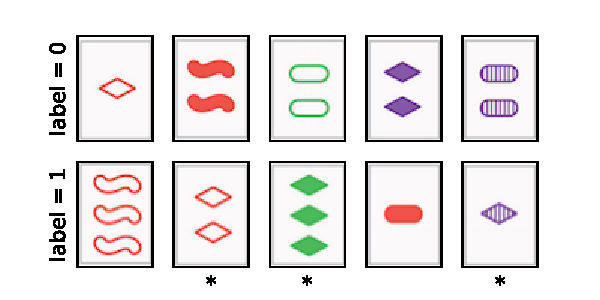
\includegraphics[width=0.9\textwidth]{figs/contains_set_example.pdf}
        \caption{Example of ``contains set'' task.}\label{fig:contains_set_example}
    \end{subfigure}
    \begin{subfigure}[b]{0.49\textwidth}
        \centering
        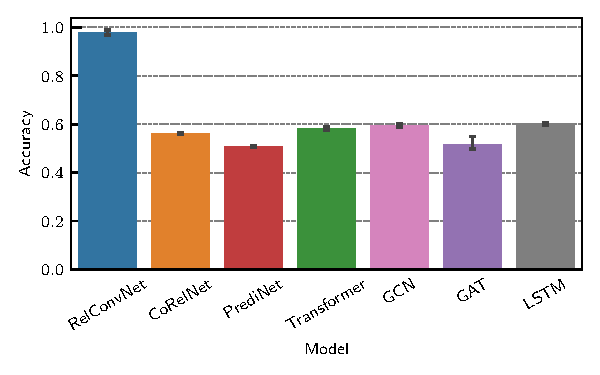
\includegraphics[width=0.9\textwidth]{figs/experiments/contains_set_acc.pdf}
        \vskip-5pt
        \caption{\footnotesize{Hold-out test accuracy.}}\label{fig:contains_set_acc}
    \end{subfigure}

    \begin{subfigure}[t]{0.97\textwidth}
        \centering
        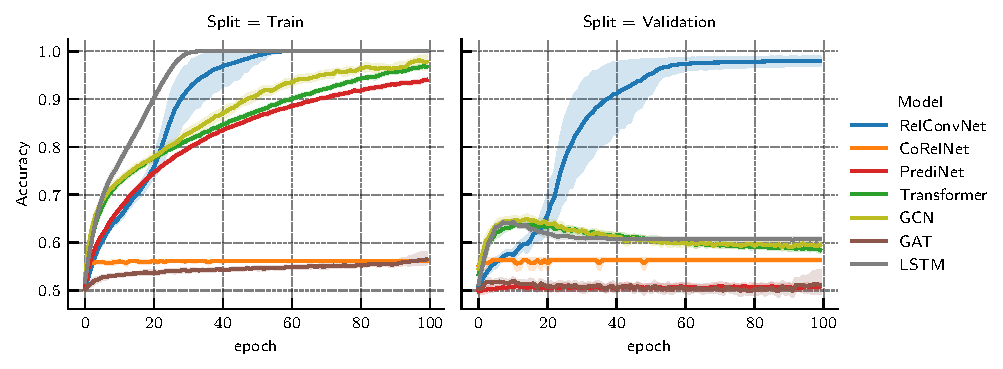
\includegraphics[width=\textwidth]{figs/experiments/contains_set_training_curves.pdf}
        \caption{Training accuracy and validation accuracy over the course of training.}\label{fig:contains_set_training_curves}
    \end{subfigure}
    % \begin{subfigure}[t]{0.45\textwidth}
    %     \centering
    %     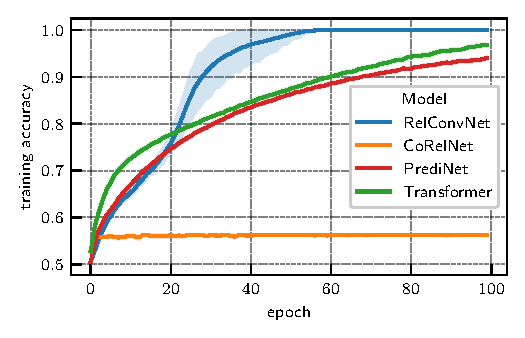
\includegraphics[width=0.9\textwidth]{figs/experiments/contains_set_training_curves_trainacc.pdf}
    %     \vskip-5pt
    %     \caption{Training accuracy over the course of training.}\label{fig:contains_set_training_curves_trainacc}
    % \end{subfigure}
    % \begin{subfigure}[t]{0.45\textwidth}
    %     \centering
    %     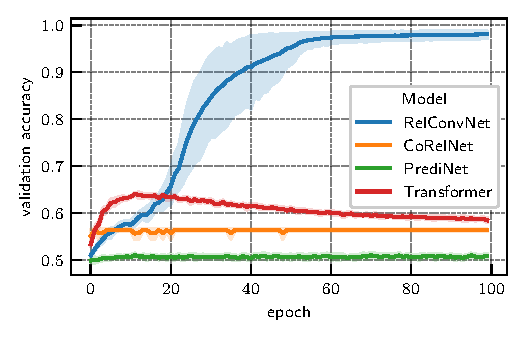
\includegraphics[width=0.9\textwidth]{figs/experiments/contains_set_training_curves_valacc.pdf}
    %     \vskip-5pt
    %     \caption{Validation accuracy over the course of training.}\label{fig:contains_set_training_curves_valacc}
    % \end{subfigure}
    \caption{Results of ``contains set'' experiments. Bar height/solid lines indicate the mean over 10 trials and error bars/shaded regions indicate 95\% bootstrap confidence intervals.}\label{fig:contains_set_experiment}
    \vskip-12.5pt
\end{figure}

We observe a sharp separation between RelConvNet and all other baselines. While RelConvNet is able to learn the task and generalize to new `sets' with near perfect accuracy (97.9\%), no other model is able to reach generalization accuracy much better than random guessing (next best is the LSTM with 60.2\%). Several models are able to fit the training data, reaching near-perfect training accuracy, but they are unable to ``learn the rule'' in a way that generalizes to the validation or test sets. This suggests that while these models are powerful function approximators, they lack the inductive biases to learn hierarchical relations.

It is perhaps surprising that models like GNNs and Transformers perform poorly on such relational tasks, given their apparent ability to process relations through neural message-passing and attention, respectively. Although GNNs are what is typically thought of in the context of ``relational'' machine learning models, they operate in a different domain compared to relational models like RelConvNet (and PrediNet, CoRelNet, etc.). In GNNs, the relations are an input to the model, received in the form of a graph, and are used to dictate the flow of information in a neural message-passing operation. By contrast, in relational convolutional networks, the input is simply a set of objects without relations---the relations need to be \textit{inferred} as part of the feature representation process. Thus, GNNs operate in domains where relational information is already present (e.g., analysis of social networks, biological networks, etc.), whereas our framework aims to solve tasks which rely on relations but those relations need to be inferred end-to-end. This offers an explanation for the poor performance of GNN baselines in this experiment---GNNs are good at processing network-style relations, but cannot infer and hierarchically process relations when they are not given. Similarly, in a Transformer, relations are modeled implicitly to direct information retrieval, but are not encoded explicitly in the resulting representations.

Models like CoRelNet and PrediNet have relational inductive biases, but lack compositionality. On the other hand, deep models like Transformers and RNNs are compositional, but lack relational inductive biases. These experiments suggest that \textit{compositionality and relational inductive biases are both necessary ingredients to efficiently learn representations of higher-order relations}. RelConvNet is a compositional architecture imbued with relational inductive biases, with the ability to tackle hierarchical relational tasks.

% We observe that RelConvNet is able to learn the task and generalize to new `sets' with near-perfect accuracy. On the other hand, CoRelNet and the Transformer have accuracies only slightly better than random guessing on the test set, while PrediNet learns nothing that generalizes to the test set. The picture becomes more clear when looking at training curves. While the Transformer and PrediNet are eventually able to fit the training data, they are unable to ``learn the rule'' in a way that generalizes to the validation or test sets. This suggests that the Transformer architecture has the general-purpose function-approximation capabilities to fit a wide array of sequence-tasks, but it does not have the right inductive biases for specialized relational reasoning. A possible explanation is that relations are processed only implicitly through its attention mechanism, rather than explicitly via a relation tensor. Moreover, it does not naturally support reasoning about the relations between groups of objects. These are strengths of the relational convolutional networks architecture.